%kelompok 5 Arsitektur Komputer
%Tiara Rizki Wulansari (1154026)
%M. A. Faris 1174041
%Evietania Charis Sujadi 1174051
%Iqbal Panggabean 1174063
%Hagan Rowlenstino 1174040
%Irvan Rizkiansyah 1174043

\section {Hexadecimal dan Binary}


\subsection {Hexadecimal}
Sistem bilangan heksadesimal (bilangan dasar 16) merepresentasikan angka yang menggunakan angka sebanyak seperempat digit sebagai sistem biner. Konversi antara heksadesimal dan biner sangat mudah sehingga hex bisa dianggap sebagai singkatan dari biner. Sistem heksadesimal membutuhkan 16 digit. Angka 0, 1, 2, 3, 4, 5, 6, 7, 8, dan 9 digunakan seperti pada sistem desimal A, B, C, D, E, dan F yang digunakan untuk bilangan desimal sesuai dengan kekuatan 16. Angka 0, 1, 2, 3, 4, 5, 6, 7, 8, dan 9 digunakan seperti pada sistem desimal A, B, C, D, E, dan F yang digunakan untuk bilangan desimal sesuai dengan kekuatan 16. Fro kanan ke kiri, yang 1's, 6's, 256's dan seterusnya. Nilai hex number 9D7A adalah 40314 dalam desimal, karena:
=======
	\subsection {Hexadecimal}
	Sistem bilangan heksadesimal (bilangan dasar 16) merepresentasikan angka yang menggunakan angka sebanyak seperempat digit sebagai sistem biner. Konversi antara heksadesimal dan biner sangat mudah sehingga hex bisa dianggap sebagai singkatan dari biner. Sistem heksadesimal membutuhkan 16 digit. Angka 0, 1, 2, 3, 4, 5, 6, 7, 8, dan 9 digunakan seperti pada sistem desimal A, B, C, D, E, dan F yang digunakan untuk bilangan desimal sesuai dengan kekuatan 16. Angka 0, 1, 2, 3, 4, 5, 6, 7, 8, dan 9 digunakan seperti pada sistem desimal A, B, C, D, E, dan F yang digunakan untuk bilangan desimal sesuai dengan kekuatan 16. Fro kanan ke kiri, yang 1's, 6's, 256's dan seterusnya. Nilai hex number 9D7A adalah 40314 dalam desimal, karena \cite{detmer2001introduction}:

	\begin{verbatim}

		 9	X	4096	36864	[	4096 = 16(3)]
	+	13	X	 256	 3328	[	D is 13, 256 = 16(2)]
	+	 7	X	  16	  112
	+	10	X	   1	   10	[	A is 10	]
						= 40314
	\end{verbatim}
Hexadecimal atau juga bisa disebut dengan sistem bilangan basis 16 adalah sistem bilangan yang menggunakan 16 simbol. berbeda dengan sistem bilangan desimal. Simbol yang digunakan dari sistem ini adalah angka 0 sampai 9, ditambah dengan 6 simbol lainnya dari huruf A sampai F. Sistem bilangan ini digunakan untuk menampilkan nilai alamat memori dalam pemrograman komputer\cite{hutahaean2015konsep}.
ciri ciri bilangan hexadecimal adalah :

	\begin{itemize}
		\item Bilangan hexadecimal memiliki bilangan basis 16
		\item Mempunyai 16 kemungkinan digit yang terbentuk
		\item Menggunakan angka dan huruf seperti (0-9) dan (A-F),huruf A-F untuk merepresentasikan 10-15
		\item Setiap digitnya merupakan bilangan pangkat 16 yang diasosiasikan berdasarkan posisinya.
	\end{itemize}

	\subsection {Penjumlahan Hexadecimal}
penjumlahan bilangan hexadecimal harus dijumlahkan berurutan dari digit yang paling kanan. Bagi 2 bilangan yang dijumlahkan, kalau hasil dari penjumlahannya lebih dari 15 maka akan menjadi carry 1, lalu hasil dari penjumlahan tersebut dikurangi 16 yang akan menjadi hasil dari penjumlahan hexadecimal.
Untuk lebih mudahnya ikuti langkah- langkah ini:
		\begin{enumerate}
			\item Tambahkan masing- masing kolom secara desimal.
			\item Kemudian ubah hasil desimal tadi menjadi heksadesimal.
			\item Lalu tuliskan hasil dari digit paling kanan dan hasil hexadesimal.
			\item Jika hasil pertambahan tiap- tiap kolom terdiri dari 2 digit, maka digit yang berada pada posisi yang paling kiri merupakan carry of untuk pertambahan kolom berikutnya.
		\end{enumerate}
			
Perhatikan contoh dibawah
\begin{verbatim}
153(16) + 234(16) = .......... (16) 
Langkah-langah penyelesainnya
153 
234 
---- (+)

1. 3 + 4 = 7
2. 5 + 3 = 8
3. 1 + 2 = 3

Karena tidak terdapat carry, maka 153(16) + 234(16) = 387(16)
\end{verbatim}
Contoh soal Lagi 
\begin{verbatim}
1A7(16) + D89(16) = .......... (16)
Langkah-langkah penyelesaiannya
1A7
D89
---- (+)

	7 + 9 = 16, karena lebih dari 15, maka terjadi carry 1 dan hasil penjumlahan adalah 0 yaitu dari 16-16.
	1 + A + 8, angka 1 adalah carry dari penjumlahan sebelumnya. A= 10 pada bilangan Decimal, jadi 1 + A + 8 = 1 + 10 + 8 = 19, hasil penjumlahan adalah 3 yatiu dari 19-16 dan carry 1.
\end{verbatim}

\subsection {Biner}
Di dalam sistem komunikasi digital modern, dimana data ditransmisikan dalam bentuk bit-bit biner, dibutuhkan sistem yang tahan terhadap noise yang terdapat di kanal transmisi sehingga data yang ditransmisikan tersebut dapat diterima dengan benar. Kesalahan dalam pengiriman atau penerimaan data merupakan permasalahan yang mendasar yang memberikan dampak yang sangat signifikan pada sistem komunikasi
Komputer menggunakan bit (digit biner, sebuah keadaan elektronik yang mewakili angka nol dan satu) untuk menunjukkan nilai. kami mewakili bilangan biner seperti itu dengan menggunakan angka 0 dan 1 sistem nilai 2 tempat. Sistem bilangan biner ini seperti sistem desimal kecuali bahwa posisi (kanan ke kiri) adalah 1, 2, 3, 4, 8, 16 (dan kekuatan yang lebih tinggi dari 2) bukan 1, 10, 100, 1000, 10000 (kekuatan 10). Sebagai contoh , bilangan biner 1101 dapat diartikan sebagai angka desimal 13\cite{dosen2013matematika}.
		\begin{verbatim}
			1			1			0			1
		one 8	  +	 one 4	  +	  one 2    +   one 1 	= 13
		\end{verbatim}
	Nomor pada  biner begitu panjang sehingga mereka canggung  untuk membaca dan juga menulis. Misalnya saja, di butuhkan 8 bit yaitu  11111010 untuk mewakili angka 250, atau 16 bit yaitu 111010100110000 untuk mewakili bilangan desimal 30000.


\subsection {Penjumlahan Biner}
Bilangan biner dapat juga dilakukan penambahan, pengurangan, perkalian dan pembagian. Kali ini, kelompok ini akan membahas tentang penjumlahan bilangan biner. Berikut adalah tata cara atau aturan penjumlahan bilangan biner :
Untuk penjumlahan operasi biner biasa, adalah operasi yang bersifat komutatif, karena untuk sembarang bilangan seperti x dan y, berlaku \verb|y+x = x+y.| Operasi penjumlahan bersifat asosiatif, karena untuk x,y,dan z yang sembarang, berlaku \verb|x+(y+z)=(x+y)+z.| \verb|Identitas yang berlaku di operasi penjumlahan ini adalah 0 (nol). Dan invers penjumlahan untuk bilangan sembarang x adalah -x, karena x+(-X)=0.|

\begin{verbatim}
	A0 + B0 = ∑0 + Cout
	Di dalam melakukan sebuah penjumlahan biasanya akan selalu melibatkan penjumlahan dengan carry in.

	Di dalam Penjumlahan Biner sendiri Ada 4 kondisi yaitu
	(0+0, 1+0, 0+1, 1+1) dimana

	0 + 0 = 0
	1 + 0 = 1
	0 + 1 = 1
	1 + 1 = 0 (carry out) 
\end{verbatim}
	Untuk maksud dari Carry out sendiri adalah hasilnya tidak bisa memuat lebih dari 1 digit. Tetapi  hasil tadi disimpan kedalam kolom sebelah yang lebih tinggi nilainya.
\begin{verbatim}
	Berikut contoh pada sebuah bilangan desimal
	7 + 2 = 9 (CarryOut = 0)
	8 + 15 = 23 (CarryOut = 1)
	Maksud dari Carry Out itu sendiri adalah penyimpangan angka, berdasarkan contoh di atas. 7 + 2 = 9 CarryOut = 0 sebab tidak ada bilangan yang di simpan. 8 + 15 = 23 bersisa 1, 1 nya ini di gantung di atas, kemudian  1 + 1 = 2, jadi hasilnya adalah 23. angka 1 yang di gantung di atas itulah yang di sebut dengan CarryOut. Dengan mengikuti atau penjumlahan- penjumlahan yang sudah tertera di atas, kita juga dapat melakukan penjummlahan biner seperti yang di tunjukkan di bawah ini.
\end{verbatim}
	Contoh pada sebuah bilangan biner :
	\begin{verbatim}
		\begin{itemize}
		\item 10 + 10 ( 1 dan 0 ) =
		  1 = CarryOut
		  10
		  10
		  __+
		  100
		\item 1 1111 (\"simpanan 1\" ingat kembali aturannya)
		  01011011 (adalah bilangan biner untuk angka 91)
		  01001110 (adalah bilangan biner untuk angka 78)
		  -------- +
		  10101001 (adalah jumlah dari 91 + 78 = 169)
		\end{itemize}
	\end{verbatim}

			\begin{figure} [ht]
				\centerline{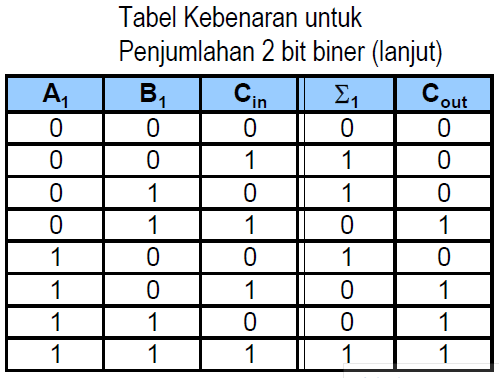
\includegraphics[width=1\textwidth]{figures/Biner2angka.png}}
				\caption{Biner2angka}
				\label{Biner2angka}
			\end{figure}
Gambar \ref{Biner2angka} ini adalah Tabel Kebeneran untuk Penjumlahan 2 bit biner.

	Apabila dalam penjumlahan biner terdapat bawaan (carry), maka akan dijumlahkan dengan tingkatan diatasnya.
	Hexadecimal atau juga bisa disebut dengan sistem bilangan basis 16 adalah sistem bilangan yang menggunakan 16 simbol. berbeda dengan sistem bilangan desimal. Simbol yang digunakan dari sistem ini adalah angka 0 sampai 9, ditambah dengan 6 simbol lainnya dari huruf A sampai F. Sistem bilangan ini digunakan untuk menampilkan nilai alamat memori dalam pemrograman komputer\cite{nurhayati2010aritmatik}.
	ciri ciri bilangan hexadecimal adalah :

	\begin{itemize}
		\item Bilangan hexadecimal memiliki bilangan basis 16
		\item Mempunyai 16 kemungkinan digit yang terbentuk
		\item Menggunakan angka dan huruf seperti (0-9) dan (A-F),huruf A-F untuk merepresentasikan 10-15
		\item Setiap digitnya merupakan bilangan pangkat 16 yang diasosiasikan berdasarkan posisinya.
	\end{itemize}

	\subsection {Penjumlahan Hexadecimal}
	penjumlahan bilangan hexadecimal harus dijumlahkan berurutan dari digit yang paling kanan. Bagi 2 bilangan yang dijumlahkan, kalau hasil dari penjumlahannya lebih dari 15 maka akan menjadi carry 1, lalu hasil dari penjumlahan tersebut dikurangi 16 yang akan menjadi hasil dari penjumlahan hexadecimal.
	Untuk lebih mudahnya ikuti langkah- langkah ini:
		\begin{enumerate}
			\item Tambahkan masing- masing kolom secara desimal.
			\item Kemudian ubah hasil desimal tadi menjadi heksadesimal.
			\item Lalu tuliskan hasil dari digit paling kanan dan hasil hexadesimal.
			\item Jika hasil pertambahan tiap- tiap kolom terdiri dari 2 digit, maka digit yang berada pada posisi yang paling kiri merupakan carry of untuk pertambahan kolom berikutnya.
		\end{enumerate}
			\begin{figure} [ht]
				\centerline{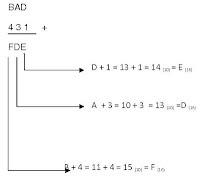
\includegraphics[width=1\textwidth]{figures/penjumlahanheksa.jpg}}
				\caption{penjumlahanheksa}
				\label{penjumlahanheksa}
			\end{figure}
	Gambar \ref{penjumlahanheksa} ini adalah penjelasan tentang penjumlahan Heksadecimal.		
	Perhatikan contoh dibawah
\begin{verbatim}
	153(16) + 234(16) = .......... (16) 
	Langkah-langah penyelesainnya
	153 
	234 
	---- (+)

	1. 3 + 4 = 7
	2. 5 + 3 = 8
	3. 1 + 2 = 3

	Karena tidak terdapat carry, maka 153(16) + 234(16) = 387(16)
\end{verbatim}
	Contoh soal Lagi 
\begin{verbatim}
	1A7(16) + D89(16) = .......... (16)
	Langkah-langkah penyelesaiannya
	1A7
	D89
	---- (+)

		7 + 9 = 16, karena lebih dari 15, maka terjadi carry 1 dan hasil penjumlahan adalah 0 yaitu dari 16-16.
		1 + A + 8, angka 1 adalah carry dari penjumlahan sebelumnya. A= 10 pada bilangan Decimal, jadi 1 + A + 8 = 1 + 10 + 8 = 19, hasil penjumlahan adalah 3 yatiu dari 19-16 dan carry 1.
\end{verbatim}	
	

\section {Biner}
=======
	Selain dengan menggunakan cara yang ada di atas, bisa juga dengan menggunakan cara pertambahan atau penjumlahan bilangan heksadesimal dengan menggunakan tabel yang ada di bawah ini \ref{tabel-pertambahan-bilangan-hexadesimal}
			\begin{figure} [ht]
				\centerline{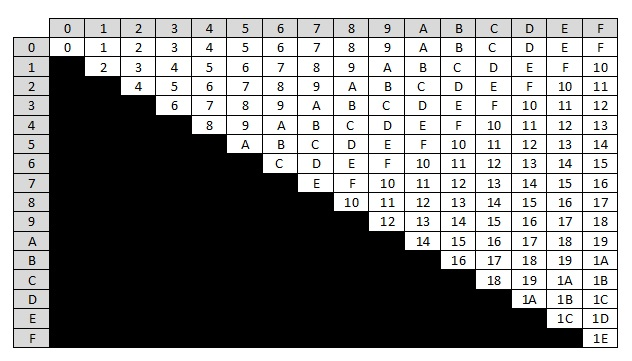
\includegraphics[width=1\textwidth]{figures/tabel-pertambahan-bilangan-hexadesimal.jpg}}

\caption{Tabel Penjumlahan Heksa}
				\label{Tabel-Penjumlahan-Heksa}
			\end{figure}

\subsection {Biner}

	Di dalam sistem komunikasi digital modern, dimana data ditransmisikan dalam bentuk bit-bit biner, dibutuhkan sistem yang tahan terhadap noise yang terdapat di kanal transmisi sehingga data yang ditransmisikan tersebut dapat diterima dengan benar. Kesalahan dalam pengiriman atau penerimaan data merupakan permasalahan yang mendasar yang memberikan dampak yang sangat signifikan pada sistem komunikasi
	Komputer menggunakan bit (digit biner, sebuah keadaan elektronik yang mewakili angka nol dan satu) untuk menunjukkan nilai. kami mewakili bilangan biner seperti itu dengan menggunakan angka 0 dan 1 sistem nilai 2 tempat. Sistem bilangan biner ini seperti sistem desimal kecuali bahwa posisi (kanan ke kiri) adalah 1, 2, 3, 4, 8, 16 (dan kekuatan yang lebih tinggi dari 2) bukan 1, 10, 100, 1000, 10000 (kekuatan 10). Sebagai contoh , bilangan biner 1101 dapat diartikan sebagai angka desimal 13\cite{detmer2001introduction}.
		\begin{verbatim}
			1			1			0			1
		one 8	  +	 one 4	  +	  one 2    +   one 1 	= 13
		\end{verbatim}
	Nomor pada  biner begitu panjang sehingga mereka canggung  untuk membaca dan juga menulis. Misalnya saja, di butuhkan 8 bit yaitu  11111010 untuk mewakili angka 250, atau 16 bit yaitu 111010100110000 untuk mewakili bilangan desimal 30000.


\subsection {Penjumlahan Biner}
Bilangan biner dapat juga dilakukan penambahan, pengurangan, perkalian dan pembagian. Kali ini, kelompok ini akan membahas tentang penjumlahan bilangan biner. Berikut adalah tata cara atau aturan penjumlahan bilangan biner :
Untuk penjumlahan operasi biner biasa, adalah operasi yang bersifat komutatif, karena untuk sembarang bilangan seperti x dan y, berlaku \verb|y+x = x+y.| Operasi penjumlahan bersifat asosiatif\cite{brent1970addition}, karena untuk x,y,dan z yang sembarang, berlaku \verb|x+(y+z)=(x+y)+z.| \verb|Identitas yang berlaku di operasi penjumlahan ini adalah 0 (nol). Dan invers penjumlahan untuk bilangan sembarang x adalah -x, karena x+(-X)=0.|
\begin{verbatim}
	A0 + B0 = ∑0 + Cout
	Di dalam melakukan sebuah penjumlahan biasanya akan selalu melibatkan penjumlahan dengan carry in.

	Di dalam Penjumlahan Biner sendiri Ada 4 kondisi yaitu
	(0+0, 1+0, 0+1, 1+1) dimana

	0 + 0 = 0
	1 + 0 = 1
	0 + 1 = 1
	1 + 1 = 0 (carry out) 
\end{verbatim}
	Untuk maksud dari Carry out sendiri adalah hasilnya tidak bisa memuat lebih dari 1 digit. Tetapi  hasil tadi disimpan kedalam kolom sebelah yang lebih tinggi nilainya.
\begin{verbatim}
	Berikut contoh pada sebuah bilangan desimal
	7 + 2 = 9 (CarryOut = 0)
	8 + 15 = 23 (CarryOut = 0)
	Maksud dari Carry Out itu sendiri adalah penyimpangan angka, berdasarkan contoh di atas. 7 + 2 = 9 CarryOut = 0 sebab tidak ada bilangan yang di simpan. 
\end{verbatim}
		
	Apabila dalam penjumlahan biner terdapat bawaan (carry), maka akan dijumlahkan dengan tingkatan diatasnya.

\subsection {Cara konversi bilangan biner ke desimal}

Cara mengkonversikan bilangan biner ke dalam desimal adalah yaitu dengan cara mengalikan satu persatu bilangan yang telah dipilih dengan 2 (baris bilangan biner), pangkat 0, pangkat 1 dan seterusnya, sesuai dengan banyaknya bilangan yang akan di konversikan, perhitungan nya yaitu dimulai dari bilangan yang paling kanan\cite{wang201140}.
=======
Cara mengkonversikan bilangan biner ke dalam desimal adalah yaitu dengan cara mengalikan satu persatu bilangan yang telah dipilih dengan 2 (baris bilangan biner), pangkat 0, pangkat 1 dan seterusnya, sesuai dengan banyaknya bilangan yang akan di konversikan, perhitungan nya yaitu dimulai dari bilangan yang paling kanan. 
contoh :
	\begin{verbatim}
		1011(2) =  1x23 + 0x22 + 1x21 + 1x20
				= 8 + 0 + 2 + 1
				= 11(10) 
	\end{verbatim}

\subsection{Penjumlahan pada bilangan Hexadecimal}
Penjumlahan bilangan hexadecimal dapat dilakukan secara sama dengan penjumlahan bilangan oktal, dengan langkah-langkah sebagai berikut :
	\begin{itemize}
		\item Tambahkan masing-masing kolom secara desimal
		\item Ubah dari hasil desimal ke hexadesimal
		\item Tuliskan hasil dari digit paling kanan dari hasil hexadesimal
		\item Jika hasil penjumlahan tiap-tiap kolom terdiri dari dua digit, maka digit paling kiri merupakan carry of untuk penjumlahan kolom selanjutnya.
	\end{itemize}
Contoh :
	\begin{verbatim}
		Desimal :
		2989
		1073
	\end{verbatim}

\cite{wang201140}
\cite{brent1970addition}
\cite{detmer2001introduction}
\cite{nurhayati2010aritmatik}
\cite{dosen2013matematika}
